\documentclass[a4paper, 16pt]{article}
\usepackage[slovene]{babel}
\usepackage[utf8]{inputenc}
\usepackage[T1]{fontenc}
\usepackage{lmodern}
\usepackage{multirow}
\usepackage{graphicx}
\usepackage{amsmath}
\usepackage{amssymb}
\usepackage{amsfonts}
\usepackage{graphicx}
\graphicspath{{figures/}}


\title{%
    Učinkovitost omrežij \\ 
    \large Poročilo}
\date{2020\\ November}
\author{Jure Babnik \\  Zala Stopar Špringer}

\begin{document}

\maketitle
\pagenumbering{gobble}


\newpage

\tableofcontents

\newpage
\pagenumbering{arabic}

\section{Priprava okolja}

Pred začetkom simulacij sva si pripravila delovno okolje. Za programerski del naloge sva uporabila \emph{Python}
in knjižnico \emph{Graph-Theory}.\\ 
Defirirala sva si funkcije, ki so nama ustvarile različne enostavne grafe, kot so mreže, 3-dimenzionalne mreže, 
popolna binomska drevesa, cikle, itd. Vsi grafi so neusmerjeni. Nato pa sva si še definirala funkcijo \emph{generate\_random}, 
ki sprejme število vozlišč $n$, na katerih funkcija naredi naključen usmerjen graf.\\
Prav tako sva si napisala funkcije, ki izračunajo učinkovitost omrežja. \\
\\
Formula za \textbf{povprečno učinkovitost} grafa $G$ je definirana kot:
$$ E(G) = \frac{1}{n(n-1)} \sum_{i\neq j \in G} \frac{1}{d(i,j)},$$

kjer je $d(i,j)$ dolžina najkrajše poti med $i$-to in $j$-to točko, $n$ pa je število vseh točk v grafu.\\
\\
\textbf{Globalna učinkovitost} je definirana kot:
$$ E_{glob}(G) = \frac{E(G)}{E(K_n)}, $$

kjer $K_n$, predstavlja poln graf na $n$ točkah.\\
\\
\textbf{Lokalna učinkovitost} je definirana kot:
$$ E_{loc}(G) = \frac{1}{n} \sum_{i \in G} E(G_i), $$

kjer $G_i$ predstavlja podgraf grafa $G$, ki je sestavljen le iz sosedov točke $i$ (brez točke $i$). \\

Vsa koda je zbrana v datoteki \emph{graphs.py}

\newpage

\section{Povprečna učinkovitost v preprostih grafih}
Ustvarila sva nekaj preprostih grafov različnih oblik in velikosti. 
Po zgornji formuli sva izračunala povprečno učinkovitost posameznega grafa in rezultate med seboj primerjala.
Zanimalo naju je predvsem, kaj se dogaja z učinkovitostjo, ko povečujemo število vozlišč.
Poleg tega pa želiva primerjati učinkovitosti grafov z enakim (podobnim) številom točk in različnih oblik.



    \subsection{Mreže $m \times n$}
    

    \begin{table}[!h]
        \begin{tabular}{c|c|c|c|c|c|c|c}
            \multirow{2}{*}{$n$} & 
            \multicolumn{7}{c}{Povprečna učinkovitost}\\
               & $m=1$       & $m=2$           & $m=3$           & $m=4$         & $m = 5$     & $m = 10$    & $m=20$     \\ \hline
            2  & $1$         & $0.83333333$ & $0.7111111$ & $0.625$       & $0.5607404$ & $0.3842982$ & $0.2500188$\\
            3  & $0.8333333$ & $0.7111111$  & $0.6157407$ & $0.5464646$   & $0.4938095$ & $0.3453350$ & $0.2285143$\\
            4  & $0.7222222$ & $0.625$      & $0.5464646$ & $0.4883333$   & $0.4436090$ & $0.3150960$ & $0.2114040$\\
            5  & $0.6416667$ & $0.5607407$  & $0.4938095$ & $0.4436090$   & $0.4046429$ & $0.2910526$ & $0.1975453$\\
            10 & $0.4286596$ & $0.3842982$  & $0.3453350$ & $0.3150960$   & $0.2910526$ & $0.2176605$ & $0.1539108$\\
            20 & $0.2734463$ & $0.2500188$  & $0.2285143$ & $0.2114040$   & $0.1975453$ & $0.1539108$ & $0.1133842$\\

        \end{tabular}
        \caption{Povprečna učinkovitost $m \times n$ mrež}
        \label{table: 1}
    \end{table}


    \subsection{3-dimenzionalne mreže}
    \begin{table}[!h]
        \begin{tabular}{c|c|c|c|c||c|c|c|c}
            \multirow{2}{*}{$n$} & 
            \multicolumn{4}{c}{$r = 2$} & \multicolumn{4}{c}{$r = 3$}\\
               & $m=2$       & $m=3$       & $m=5$       & $m=10$      & $m = 2$     & $m = 3$    & $m=5$        & $m=10$ \\ \hline
            2  & $0.6904761$ & $0.5959596$ & $0.4782456$ & $0.3357206$ & $0.5959596$ & $0.5193800$ & $0.4223864$ & $0.3018993$\\
            3  & $0.5959596$ & $0.5193800$ & $0.4223864$ & $0.3018993$ & $0.5193800$ & $0.4562206$ & $0.3753992$ & $0.2728478$\\
            5  & $0.4782456$ & $0.4223864$ & $0.3498866$ & $0.2565895$ & $0.4223864$ & $0.3753992$ & $0.3141630$ & $0.2339359$ \\
            10 & $0.3357206$ & $0.3018993$ & $0.2565895$ & $0.1954146$ & $0.3018993$ & $0.2728478$ & $0.2339359$ & $0.1805703$\\

        \end{tabular}
        \caption{Povprečna učinkovitost $m \times n \times r$ mrež}
        \label{table: 2}
    \end{table}

    \begin{table}[!h]
        \begin{tabular}{c|c|c|c|c||c|c|c|c}
            \multirow{2}{*}{$n$} & 
            \multicolumn{4}{c}{$r = 5$} & \multicolumn{4}{c}{$r = 10$}\\
               & $m=2$       & $m=3$       & $m=5$       & $m=10$      & $m = 2$     & $m = 3$     & $m=5$       & $m=10$ \\ \hline
            2  & $0.4782456$ & $0.4223864$ & $0.3498866$ & $0.2565895$ & $0.3357206$ & $0.3018993$ & $0.2565895$ & $0.1954146$\\
            3  & $0.4223864$ & $0.3753992$ & $0.3141630$ & $0.2339359$ & $0.3018993$ & $0.2728478$ & $0.2339359$ & $0.1805793$\\
            5  & $0.3498866$ & $0.3141630$ & $0.2669560$ & $0.2032711$ & $0.2565895$ & $0.2339359$ & $0.2032711$ & $0.1600518$\\
            10 & $0.2565895$ & $0.2339359$ & $0.2032711$ & $0.1600518$ & $0.1954146$ & $0.1805703$ & $0.1600518$ & $0.1298527$\\

        \end{tabular}
        \caption{Povprečna učinkovitost $m \times n \times r$ omrežij}
        \label{table: 3}
    \end{table}

\newpage

    \subsection{Cikli}
    \begin{table}[!h]
        \begin{tabular}{c|c}
            n & Povprečna učinkovitost \\ \hline
            3   & $1$ \\
            4   & $0.8333333$ \\
            5   & $0.75$ \\
            10  & $0.4851852$ \\
            20  & $0.3030493$ \\
            50  & $0.1549371$ \\
            100 & $0.0906910$ \\

        \end{tabular}
        \caption{Povprečna učinkovitost ciklov z $n$ točkami}
        \label{table: 4}
    \end{table}

    \subsection{Binomska drevesa}
    \begin{table}[!h]
        \begin{tabular}{c|c}
            n & Povprečna učinkovitost \\ \hline
            2  & $0.8333333$ \\
            3  & $0.5634921$ \\
            4  & $0.3907937$ \\
            5  & $0.2776549$ \\
            6  & $0.2028584$ \\
            7  & $0.1530067$ \\
            8  & $0.1193636$ \\
            9  & $0.0962377$ 

        \end{tabular}
        \caption{Povprečna učinkovitost popolnih binomskih dreves globine $n$}
        \label{table: 5}
    \end{table}

    \subsection{Primerjava}
    Najprej primerjamo mreže oblike $1\times n$ s cikli dolžine $n$. So namreč zelo podobne oblike, 
    razlikujejo pa se v eni sami povezavi, ki je prisotna le v ciklu. Do razlike v učinkovitosti pride
    ravno zaradi te povezave. Če si za primer izberemo $n = 3$ opazimo, da je v ciklu poljuben par vozlišč
    med seboj oddaljen $1$ povezavo, medtem ko se v mreži dimenzije $3\times 1$ pojavi par, ki je oddaljen $2$ povezavi.
    Ker se v formuli razdalja med parom vozlišč pojavlja v imenovalcu, večja razdalja pomeni manjšo učinkovitost.
    Poleg tega se v primeru cikla zaradi dodatne povezave pot med marsikaterim parom točk skrajša. Tudi najini izračuni 
    povejo enako zgodbo. Če si spet pogledmo kot primer $n = 3$, ima cikel povprečno učinkovitost $1$, mreža
    pa le $0.833$. Tudi za večje grafe, npr. $n = 20$, opazimo razliko; cikel ima poveprečno učinkovitost $0.303$, 
    mreža pa le $0.273$.\\

    Podobna pričakovanja sva imela glede primerjave med mrežami oblike $1 \times n$ ter $m \times n$ (na enakem številu točk).
    Mreže z več povezavami so zaradi podobnega premisleka kot v prejšnjem primeru bolj učinkovite. 
    Če si primerjamo npr. mrežo $10 \times 1$ z mrežo $5 \times 2$ opazimo, da ima kljub enakemu številu točk slednja učinkovitost
    $0.561$, kar je več kot $0.273$ (učinkovitost mreže $10 \times 1$).\\

    Podobno, če za primer vzamemo mreži dimenzij $10 \times 2$ in $5 \times 4$, lahko iz tabele razberemo, da ima tabela dimenzije
    $5 \times 4$ večjo učinkovitost, kljub enakemu številu točk. \\

    Kot nadaljevanje prejšnje točke sva primerjala tudi 2-dimenzionalne mreže s 3-dimenzionalnimi. Pričakovala sva
    podoben rezultat; da so 3-dimenzionalne bolj učinkovite od 2-dimenzionalnih. Predvidevanje se je izkazalo za resnično.
    2-dimenzionalne mreže dimenzije $m \times n$ lahko razumemo kot 3-dimenzionalno dimenzij $1 \times m \times n$. Po podobnem 
    premisleku kot v primerjavi mrež $1 \times n$ z $m \times n$ rezultat ni nobeno presenečenje.

    Nazadnje sva primerjala še mreže z binomskimi drevesi. Zaradi povsem različne strukture obeh grafov nisva bila povsem prepričana,
    kakšne rezultate naj pričakujeva. Vseeno pa sva se rahlo nagibala v prid mrež, saj imajo več povezav. Rezultati so najino hipotezo
    podprli. Za primer vzamemo mrežo dimenzije $3 \times 5$ ter binomsko drevo višine $4$ (saj imata oba $15$ vozlišč). Mreža ima 
    učinkovtost $0.494$, drevo pa le $0.390$. Podobno ima mreža dimenzij $5 \times 5 \times 5$ $125$ točk in povprečno učinkovitost $0.267$,
    drevo višine $7$ pa $127$ točk in povprečno učinkovitost $0.153$ (torej bistveno manj).\\

    Po zgornjih ugotovitvah sva vsakič prišla do sklepa, da je graf z več povezavami bolj učinkovit. Zato sva se odločila, da bova binomska drevesa
    in mreže primerjala tako, da med seboj primerjava grafa z enakim (podobnim) številom povezav. Za začetek si poglejmo manjši primer; mreža 
    $2 \times 3$ in binomsko drevo višine $3$. Drevo ima $6$ povezav in povprečno učinkovitost $0.563$, mreža pa ima povezavo več in učinkovitost $0.711$.
    Če nato primerjamo mrežo dimenzij $2 \times 3 \times 5$ z binomskim drevesom višine $6$, dobimo podoben rezultat; mreža ima $59$ povezav in 
    povprečno učinkovitost $0.422$, drevo pa $3$ povezave več in učinkovitost $0.202$. Je pa treba omeniti, da ima mreža precej manj točk kot drevo.
    



\section{Povprečna učinkovitost izračunana s približkom}
Ker je formula za računanje povprečne učinkovitosti zelo zahtevna, sva se odločila, da bova preverila, kako velika je napaka,
če povprečno učinkovitost izračunamo s približki.
Napisala sva funkcijo \emph{average\_sim}. Funkciji povemo odstotek, kolikšen delež parov toč naj vzame.
Nato funkcija izračuna povprečno učinkovitost na naključni podmnožici. \\
Za različne grafe in različno število vozlišč sva računala približke za $0.01 \%$, $0.02 \%$, $0.03 \%$, $0.04 \%$, $0.05 \%$, $0.1 \%$, $0.15 \%$, , $0.2 \%$, , $0.25 \%$ in za $0.5 \%$ parov točk.
Za vsak graf in vsak pdstotek sva postopek ponovila $10$ krat, $100$ krat in $1000$ krat ter nato izračunala povprečje dobljenih rezultatov.


\newpage

    \subsection{Mreža dimenzije $3 x 1$}
    \begin{table}[!h]
        \begin{tabular}{c|c|c|c|c}
            Procent & Povprečna učinkovitost & Približek 10 & Približek 100 & Približek 1000 \\ \hline
            $0.01$ & $0.8333$ & $0.8$  & $0.79$   & $0.815$ \\
            $0.02$ & $0.8333$ & $0.85$ & $0.825$  & $0.8405$ \\
            $0.03$ & $0.8333$ & $0.75$ & $0.81$   & $0.8365$ \\
            $0.04$ & $0.8333$ & $0.85$ & $0.86$   & $0.8405$ \\
            $0.05$ & $0.8333$ & $0.9$  & $0.855$  & $0.828$ \\
            $0.1$  & $0.8333$ & $0.75$ & $0.815$  & $0.8315$ \\
            $0.15$ & $0.8333$ & $1.0$  & $0.87$   & $0.8335$ \\
            $0.2$  & $0.8333$ & $0.85$ & $0.835$  & $0.8298$ \\
            $0.25$ & $0.8333$ & $0.8$  & $0.845$  & $0.8315$ \\
            $0.5$  & $0.8333$ & $0.85$ & $0.8383$ & $0.8322$ \\

        \end{tabular}
        \caption{Povprečna učinkovitost in približki za mrežo dimenzije $3$ $x$ $1$}
        \label{table: 6}
    \end{table}

    \subsection{Mreža dimenzije $4 \times 3 \times 2$}
    \begin{figure}[!h]
        \centering
        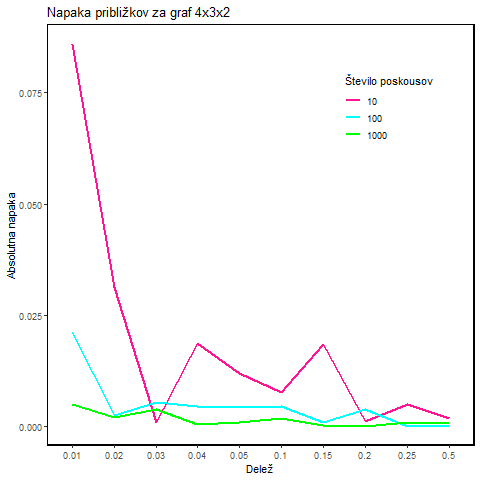
\includegraphics[width = 0.6\textwidth]{../Vizualizacija/Grid_4x3x2.png}
        \label{fig: grid}
    \end{figure}

\newpage    
    \subsection{Drevo globine $5$}
    \begin{figure}[!h]
        \centering
        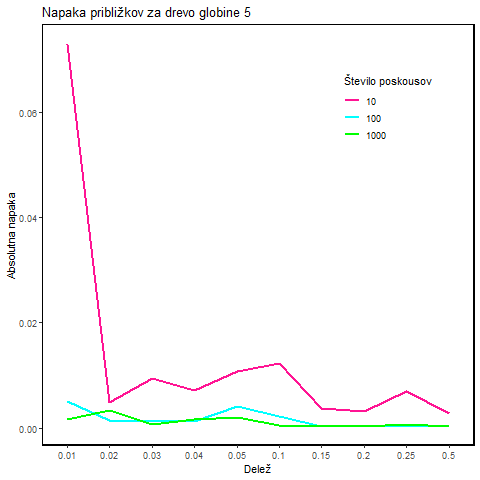
\includegraphics[width = 0.6\textwidth]{../Vizualizacija/Tree_5.png}
        \label{fig: tree}
    \end{figure}


    


\section{Globalna učinkovitost}

Zanimala naju je tudi globalna učinkovitost. Odločila sva se, da jo bova izračunala samo za 3-dimenzinalne grafe in za drevesa.
To je zato, ker so $n \times m$ mreže pravdaprav 3-dimenzionalne, s tem, da je ena dimenzija $1$, cikli pa so podobni mrežam $m \times 1 \times 1$.

\section{Sklep}
uvodna beseda\\
Po pričakovanjih povprečna učinkovitost pada z večanjem števila točk.
To se zdi smiselno, saj so v večjih omrežjih posamezni pari točk med seboj bolj oddaljeni.
Slednje velja za grafe vseh zgoraj omenjenih oblik. 
Ugotovila sva tudi, da so izmed preizkovanih omrežij najbolj učinkovite 3-dimenzionalne mreže, 
najmanj pa mreže dimenzije $n \times 1$. To je zato, ker imajo 3-dimenzionalne mreže več povezav, čeprav primerjamo grafa z enakim številom vozlišč.
S tem, ko sva primerjala binomska drevesa in mreže, sva ugotovila, da večje število povezav ne pomeni nujno večje učinkovitosti. 
Iz najinih izračunov sklepava, da so najbolj učinkoviti tisti grafi, pri katerih je posamezno vozlišče povezano s čim več ostalimi. 
Za primer lahko uzamemo poln graf, ki ima povprečno učinkovitost vedno enako $1$.






\end{document}